\appendix

\section{NLO QED corrections in APFEL} \label{sec:appendixAPFEL}

In this appendix we present the details of the implementation of the
joint NLO QCD+QED corrections in {\tt APFEL}.
%
As discussed in~\cite{Bertone:2013vaa},
the implementation of LO
QED effects presents many simplifications,
in particular the fact that QED and QCD
corrections do not mix, and therefore the DGLAP evolution
equations as well as the
$\alpha_s$ and $\alpha$ running are decoupled.
%
On the other hand,
when going
to NLO this property does not
hold anymore,
and there QED and QCD contributions mix both in the DGLAP and in the
coupling evolution equations.
%
On top of this complication, these mixed corrections induce
the presence of diagrams in which a real photon is present either in
the initial or in the final state and that have to be included in the
computation of the DIS structure functions.

In the following we will
first discuss how to generalize the coupling evolution equations
(finding that the presence of the mixed QCD+QED terms leads to a
negligible difference in the running), we will then turn to the DGLAP,
and finally we will consider both neutral-current and charged-current
DIS structure functions.

\subsection{Evolution of the couplings}

As  mentioned above, NLO QCD+QED corrections induce the presence of
mixed terms at the level of the running of the
corresponding coupling constants.
%
That is,
the QCD $\beta$-function receives corrections proportional to $\alpha$
and, vice-versa, the QED $\beta$-function receives corrections
proportional to $\alpha_s$, in such a way that the coupling evolution
equations read:
\begin{equation}\label{CoupledEq}
\begin{array}{rcl}
\displaystyle \mu^2\frac{\partial \alpha_s}{\partial \mu^2} &=& \displaystyle
                                                \beta^{\rm QCD}(\alpha_s,\alpha)\,,\\
\\
\displaystyle \mu^2\frac{\partial \alpha}{\partial \mu^2} &=& \displaystyle \beta^{\rm QED}(\alpha_s,\alpha)\,.
\end{array}
\end{equation}
As a consequence, these evolution equations form a set of coupled
differential equations. Up to three loops ($i.e.$ NLO), the
$\beta$-functions can be expanded as:
\begin{equation}
\beta^{\rm QCD}(\alpha_s,\alpha) = -\alpha_s\left[\beta_0^{(\alpha_s)}\left(\frac{\alpha_s}{4\pi}\right)+\beta_1^{(\alpha_s\alpha)}\left(\frac{\alpha_s}{4\pi}\right) \left(\frac{\alpha}{4\pi}\right)+\beta_1^{(\alpha_s^2)}\left(\frac{\alpha_s}{4\pi}\right)^2+\dots\right]\,,
\end{equation}
and:
\begin{equation}
\beta^{\rm QED}(\alpha_s,\alpha) = -\alpha\left[\beta_0^{(\alpha)}\left(\frac{\alpha}{4\pi}\right)+\beta_1^{(\alpha\alpha_s)}\left(\frac{\alpha}{4\pi}\right) \left(\frac{\alpha_s}{4\pi}\right)+\beta_1^{(\alpha^2)}\left(\frac{\alpha}{4\pi}\right)^2+\dots\right]\,,
\end{equation}
where the ``new'' terms are the mixing terms
$\beta_1^{(\alpha_s\alpha)}$ and $\beta_1^{(\alpha\alpha_s)}$, and the
pure NLO QED term $\beta_1^{(\alpha^2)}$ have been computed in
Ref.~\cite{Surguladze:1996hx}. Taking into account a factor four due
the different definitions of the expansion parameter and writing
explicitly the color factors one finds:
\begin{equation}\label{eq:NewBetaTerms}
\beta_1^{(\alpha_s\alpha)} = -2\sum_{i=1}^{n_f}
e_q^2\,\qquad\beta_1^{(\alpha\alpha_s)} = -\frac{16}{3}N_c\sum_{i=1}^{n_f} e_q^2\,,\qquad \beta_1^{(\alpha^2)} = -4\left(n_l+N_c\sum_{i=1}^{n_f} e_q^2\right)\,.
\end{equation}
where $N_c=3$ is the number of colors, $e_q$ is the electric charge of
the quark flavour $q$, and $n_f$ and $n_l$ are the numbers of active
quark and leptons flavours, respectively.


Eq.~(\ref{CoupledEq}) can be written in the vectorial form:
\begin{equation}\label{CoupledEqVect}
\mu^2\frac{\partial {\bm \alpha}}{\partial \mu^2} = {\bm \beta}\left({\bm \alpha}(\mu)\right)\,,
\end{equation}
with:
\begin{equation}
  {\bm \alpha} = {\alpha_s \choose \alpha}\qquad\mbox{and}\qquad  {\bm \beta} = {\beta^{\rm QCD} \choose \beta^{\rm QED}}\,.
\end{equation}
Eq.~(\ref{CoupledEqVect}) is an ordinary differential equation that
can be numerically solved using the Runge-Kutta method.

The first two terms in eq.~(\ref{eq:NewBetaTerms}) are responsible for
the coupling of the evolution of $\alpha_s$ and $\alpha$ and thus they
introduce a complication that affects both the implementation and the
performance of the relative code. One can then ask what is the effect
of their presence and whether their removal makes a substantial
difference. In Fig.~\ref{fig:CouplingEvol} we show the comparison
between the evolution at NLO of both couplings $\alpha_s$ and $\alpha$
including and excluding the mixing terms in the respective
$\beta$-functions. The evolution is performed between the $Z$ mass
scale $M_Z$ and 10 TeV with 5 active quark flavours and 3 active
lepton flavours and uses as boundary conditions
$\alpha_s(M_Z) = 0.118$ and $\alpha(M_Z) = 1/128$. The two curves in
Fig.~\ref{fig:CouplingEvol} are normalised to the respective curve
without mixing terms. It is clear that the mixed terms lead to tiny
relative differences that are at most of $\mathcal{O}(10^{-4})$ at 10
TeV for $\alpha_s$ and $\mathcal{O}(10^{-3})$ at the same scale for
$\alpha$. We conclude that the mixed terms in the $\beta$-functions
have a negligible effect on the coupling evolution and thus we exclude
them to make the code simpler and improve the performance without
introducing any significant inaccuracy.

%%%%%%%%%%%%%%%%%%%%%%%%%%%%%%%%%%%%%%%%%%%%%%%%%%%%%%%%
\begin{figure}[h]
\includegraphics[width=6cm,angle=270]{figs/couplings.eps} 
\caption{Comparison between the running with the scale
$Q$ of the QCD and QED couplings,
  $\alpha_s$ and $\alpha$, including or not the mixed terms in
  the corresponding $\beta$-functions.
%
The curves are normalised to the result of the respective coupling
  running without the mixing terms.}
\label{fig:CouplingEvol}
\end{figure}
%%%%%%%%%%%%%%%%%%%%%%%%%%%%%%%%%%%%%%%%%%%%%%%%%%%%%%%%

\subsection{Impact on PDF evolution}

Next, we address the question of implementing the full NLO
QCD+QED corrections to the DGLAP evolution equations. Here we limit
ourselves to consider only the photon PDF without including the
leptons. The generalisation to the full set of PDFs can be achieved
relatively easily following the same steps discussed below.

The first step towards an efficient implementation of the solution of
the DGLAP equations in the presence of QED corrections is the adoption
of a suitable set of combinations of PDFs that diagonalize the
splitting function matrix, decoupling as many DGLAP equations as
possible. Such a set of combinations (or basis) was already introduced
in Appendix A of Ref.~\cite{Bertone:2015lqa} and will be used also
here (without considering the distributions involving leptons). The
basis reads:
\begin{equation}\label{eq:EvolBasis}
\begin{array}{ll}
\mbox{\texttt{ 1} : }g & \\
\mbox{\texttt{ 2} : }\gamma & \\
\mbox{\texttt{ 3} : }\displaystyle \Sigma = \Sigma_u + \Sigma_d & \quad
\mbox{\texttt{9} : }\displaystyle V =V_u +  V_d\\
\mbox{\texttt{ 4} : } \displaystyle \Delta_\Sigma = \Sigma_u - \Sigma_d& \quad\displaystyle 
\mbox{\texttt{10} : } \Delta_V = V_u - V_d\\
\mbox{\texttt{ 5} : }T_1^u = u^+ - c^+ &\quad \mbox{\texttt{11} : }V_1^u = u^- - c^- \\
\mbox{\texttt{ 6} : }T_2^u = u^+ + c^+ - 2t^+ &\quad \mbox{\texttt{12} : }V_2^u = u^- + c^- - 2t^-\\
\mbox{\texttt{ 7} : }T_1^d = d^+ - s^+ &\quad \mbox{\texttt{13} : }V_1^d = d^- - s^- \\
\mbox{\texttt{ 8} : }T_2^d = d^+ + s^+ - 2b^+ &\quad \mbox{\texttt{14}
                                               : }V_2^d = d^- + s^- -
                                               2b^-\\
\end{array}
\end{equation}
where we have defined $q^\pm = q\pm\overline{q}$ with
$q = u,d,s,c,b,t$ and:
\begin{equation}
\begin{array}{ll}
\Sigma_u = u^++c^++t^+, &\quad V_u = u^-+c^-+t^-,\\
\\
\Sigma_d = d^++s^++b^+,&\quad V_d = d^-+s^-+b^-\,.
\end{array}
\end{equation}
The second step is construct the splitting function matrix responsible
for the evolution of each one of the distributions defined above. To
do so, we split each splitting function $P$ into a pure QCD term
$\widetilde{P}$, which only depends on $\alpha_s$, and a QCD+QED
correction term $\bar{P}$, which instead contains contributions having
at least one power of $\alpha$ but that can also contain mixed
terms. In practice:
\begin{equation}
P = \widetilde{P} + \bar{P}\,,
\end{equation}
where:
\begin{equation}\label{eq:PureQCDSplittings}
\widetilde{P} = \alpha_s \mathcal{P}^{(1,0)} + \alpha_s^2 \mathcal{P}^{(2,0)}+\dots\,,
\end{equation}
and:
\begin{equation}\label{eq:QCD+QEDSplittings}
\bar{P} = \alpha \mathcal{P}^{(0,1)} + \alpha_s\alpha \mathcal{P}^{(1,1)}+\alpha^2 \mathcal{P}^{(0,2)}\dots
\end{equation}
Note that in the r.h.s. of both eqs.~(\ref{eq:PureQCDSplittings})
and~(\ref{eq:QCD+QEDSplittings}) we are using the notation of
Refs.~\cite{deFlorian:2015ujt,deFlorian:2016gvk} to indicate the power
of $\alpha_s$ and $\alpha$ that a given splitting function multiplies.

The structure of the pure QCD splitting function matrix
$\widetilde{P}$ as well as the first term in $\bar{P}$, which
represents the LO QED correction, in the basis given in
eq.~(\ref{eq:EvolBasis}) was discussed in
Ref.~\cite{Bertone:2015lqa}. It is now necessary to analyze the
structure of the two additional terms $\mathcal{P}^{(1,1)}$ and
$\mathcal{P}^{(0,2)}$. Let us start we the
$\mathcal{O}(\alpha_s\alpha)$ correction. The resulting evolution
equations at this order are:
\begin{equation}
\begin{array}{rcl}
\displaystyle\left.\mu^2\frac{\partial}{\partial \mu^2}
\begin{pmatrix}
g\\
\gamma\\
\Sigma\\
\Delta_\Sigma
\end{pmatrix}
\right|_{\mathcal{O}(\alpha_s \alpha)} &=& \displaystyle \begin{pmatrix}
e_\Sigma^2 \mathcal{P}^{(1,1)}_{gg}      & e_\Sigma^2 \mathcal{P}^{(1,1)}_{g\gamma} & \eta^+\mathcal{P}^{(1,1)}_{gq} & \eta^-\mathcal{P}^{(1,1)}_{gq} \\
e_\Sigma^2 \mathcal{P}^{(1,1)}_{\gamma g} & e_\Sigma^2 \mathcal{P}^{(1,1)}_{\gamma\gamma} & \eta^+\mathcal{P}^{(1,1)}_{\gamma q} &\eta^-\mathcal{P}^{(1,1)}_{\gamma q} \\
2 e_\Sigma^2 \mathcal{P}^{(1,1)}_{qg}    & 2 e_\Sigma^2 \mathcal{P}^{(1,1)}_{q\gamma} & \eta^+\mathcal{P}^{+(1,1)}  & \eta^-\mathcal{P}^{+(1,1)}\\
2 \delta_e^2 \mathcal{P}^{(1,1)}_{qg} & 2 \delta_e^2 \mathcal{P}^{(1,1)}_{q\gamma} &\eta^-\mathcal{P}^{+(1,1)} &\eta^+\mathcal{P}^{+(1,1)}
\end{pmatrix}\otimes
\begin{pmatrix}
g\\
\gamma\\
\Sigma\\
\Delta_\Sigma
\end{pmatrix}
\end{array}\,,
\end{equation}

\begin{equation}
\displaystyle\left.\mu^2\frac{\partial}{\partial \mu^2}
\begin{pmatrix}
V\\
\Delta_V
\end{pmatrix} \right|_{\mathcal{O}(\alpha_s \alpha)}= 
\begin{pmatrix}
\eta^+\mathcal{P}^{-(1,1)} & \eta^-\mathcal{P}^{-(1,1)} \\
\eta^-\mathcal{P}^{-(1,1)} & \eta^+\mathcal{P}^{-(1,1)} 
\end{pmatrix}\otimes
\begin{pmatrix}
V\\
\Delta_V
\end{pmatrix}\,,
\end{equation}

\begin{equation}
\begin{array}{ll}
\begin{array}{rcl}
\displaystyle \left.\mu^2\frac{\partial T^u_{1,2}}{\partial \mu^2}\right|_{\mathcal{O}(\alpha_s \alpha)} &=&
\displaystyle e_u^2\mathcal{P}^{+(1,1)}\otimes T^u_{1,2}
\end{array}\,, &
\begin{array}{rcl}
\displaystyle \left.\mu^2\frac{\partial T^d_{1,2}}{\partial \mu^2}\right|_{\mathcal{O}(\alpha_s \alpha)} &=&
\displaystyle e_d^2\mathcal{P}^{+(1,1)} \otimes T^d_{1,2}
\end{array}\,,
\\
\\
\begin{array}{rcl}
\displaystyle \left.\mu^2\frac{\partial V^u_{1,2}}{\partial \mu^2}\right|_{\mathcal{O}(\alpha_s \alpha)} &=&
\displaystyle e_u^2\mathcal{P}^{-(1,1)} \otimes V^u_{1,2}
\end{array}\,, &
\begin{array}{rcl}
\displaystyle \left.\mu^2\frac{\partial V^d_{1,2}}{\partial \mu^2}\right|_{\mathcal{O}(\alpha_s \alpha)} &=&
\displaystyle e_d^2\mathcal{P}^{-(1,1)}\otimes V^d_{1,2}
\end{array}\,.
\end{array}
\end{equation}
where $\otimes$ indicates the Mellin convolution and where we have
defined:
\begin{equation}
\begin{array}{rcl}
e_{\Sigma}^{2}& \equiv &\displaystyle
N_c(n_ue_{u}^{2}+n_de_{d}^{2})\,,\\
\\
\delta_e^2 & \equiv &\displaystyle N_c(n_u e_u^2 -n_d e_d^2)\,,\\
\\
\eta^{\pm} & \equiv & \displaystyle \frac{1}{2}\left(e_{u}^{2}\pm
  e_{d}^{2}\right)\,,\\
\end{array}
\end{equation}
with $e_u$ and $e_d$ the electric charges of the up- and down-type
quarks, and $n_u$ and $n_d$ the number of up- and down-type active
quark flavours (such that $n_u+n_d=n_f$).

Now we turn to consider the $\mathcal{O}(\alpha^2)$ corrections. The
explicit expressions of the splitting functions at this order are
reported in Ref.~\cite{deFlorian:2016gvk}. There are two main new
features that distinguish these expressions from the
$\mathcal{O}(\alpha)$ and $\mathcal{O}(\alpha_s\alpha)$ ones and that
are relevant to the implementation. The first is that, contrary to the
other cases in which the electric charges appeared to the second power
at the most, here they appear up to the fourth power. As a consequence
we need to introduce the new couplings:
\begin{equation}
\begin{array}{l}
+e_{\Sigma}^4 = N_c(n_{u} e_u^4 + n_{d} e_d^4)\,,\\
+\\
+\delta_e^4 = N_c(n_{u} e_u^4 - n_{d} e_d^4)\,.
\end{array}
\end{equation}

The second feature is that the dependence on the electric charges of
some of the $\mathcal{O}(\alpha^2)$ splitting functions is not
factorisable as it was the case for all the $\mathcal{O}(\alpha)$ and
$\mathcal{O}(\alpha_s\alpha)$ ones. In these cases we need to
distinguish between up-type and down-type splitting functions. After
some algebra we find that the $\mathcal{O}(\alpha^2)$ contributions to
the QCD+QED DGLAP equations read:

\begin{equation}
%\begin{array}{rcl}
\begin{array}{c}
\displaystyle\left.\mu^2\frac{\partial}{\partial \mu^2}
\begin{pmatrix}
g\\
\gamma\\
\Sigma\\
\Delta_\Sigma
\end{pmatrix}
  \right|_{\mathcal{O}(\alpha^2)} =\\
\\
 \displaystyle \frac12\begin{pmatrix}
    0 & 0 & 0 & 0 \\
    0 & 2e_\Sigma^4 \mathcal{P}_{\gamma\gamma}^{(0,2)} & e_u^4 \mathcal{P}_{\gamma
      u}^{(0,2)} + e_d^4 \mathcal{P}_{\gamma d} & e_u^4 \mathcal{P}_{\gamma u}^{(0,2)} - e_d^4 \mathcal{P}_{\gamma d}^{(0,2)}\\
    0 & 4 e_\Sigma^4 \mathcal{P}^{(0,2)}_{q\gamma} &
    e_u^4\mathcal{P}_{uu}^{+(0,2)}
    +e_d^4\mathcal{P}_{dd}^{+(0,2)}+2\eta^+e_\Sigma^2\mathcal{P}^{S(0,2)}_{qq} & e_u^4\mathcal{P}_{uu}^{+(0,2)}-e_d^4\mathcal{P}_{dd}^{+(0,2)} + 2\eta^-e_\Sigma^2\mathcal{P}^{S(0,2)}_{qq}\\
    0 & 4 \delta_e^4 \mathcal{P}^{(0,2)}_{q\gamma} & e_u^4\mathcal{P}_{uu}^{+(0,2)}
    -e_d^4\mathcal{P}_{dd}^{+(0,2)}+2\eta^-\delta_e^2
    \mathcal{P}^{S(0,2)}_{qq} & e_u^4\mathcal{P}_{uu}^{+(0,2)}+e_d^4\mathcal{P}_{dd}^{+(0,2)} + 2\eta^+\delta_e^2 \mathcal{P}^{S(0,2)}_{qq}
\end{pmatrix}\otimes
\begin{pmatrix}
g\\
\gamma\\
\Sigma\\
\Delta_\Sigma
\end{pmatrix}\,,
\end{array}
\end{equation}

\begin{equation}
\displaystyle\left.\mu^2\frac{\partial}{\partial \mu^2}
\begin{pmatrix}
V\\
\Delta_V
\end{pmatrix} \right|_{\mathcal{O}(\alpha^2)}= \frac12
\begin{pmatrix}
e_u^4\mathcal{P}_{uu}^{-(0,2)}+e_d^4\mathcal{P}_{dd}^{-(0,2)} & e_u^4\mathcal{P}_{uu}^{-(0,2)}-e_d^4\mathcal{P}_{dd}^{-(0,2)} \\
e_u^4\mathcal{P}_{uu}^{-(0,2)}-e_d^4\mathcal{P}_{dd}^{-(0,2)} & e_u^4\mathcal{P}_{uu}^{-(0,2)}+e_d^4\mathcal{P}_{dd}^{-(0,2)} 
\end{pmatrix}\otimes
\begin{pmatrix}
V\\
\Delta_V
\end{pmatrix}\,,
\end{equation}

\begin{equation}
\begin{array}{ll}
\begin{array}{rcl}
\displaystyle \left.\mu^2\frac{\partial T^u_{1,2}}{\partial \mu^2}\right|_{\mathcal{O}(\alpha^2)} &=&
\displaystyle e_u^4\mathcal{P}_{uu}^{+(0,2)}\otimes T^u_{1,2}
\end{array}\,, &
\begin{array}{rcl}
\displaystyle \left.\mu^2\frac{\partial T^d_{1,2}}{\partial \mu^2}\right|_{\mathcal{O}(\alpha^2)} &=&
\displaystyle e_d^4\mathcal{P}_{dd}^{+(0,2)} \otimes T^d_{1,2}
\end{array}\,,
\\
\\
\begin{array}{rcl}
\displaystyle \left.\mu^2\frac{\partial V^u_{1,2}}{\partial \mu^2}\right|_{\mathcal{O}(\alpha^2)} &=&
\displaystyle e_u^4\mathcal{P}_{uu}^{-(0,2)} \otimes V^u_{1,2}
\end{array}\,, &
\begin{array}{rcl}
\displaystyle \left.\mu^2\frac{\partial V^d_{1,2}}{\partial \mu^2}\right|_{\mathcal{O}(\alpha^2)} &=&
\displaystyle e_d^4\mathcal{P}_{dd}^{-(0,2)}\otimes V^d_{1,2}
\end{array}\,.
\end{array}
\end{equation}
It should be noticed that, as compared to the expressions presented in
Ref.~\cite{deFlorian:2016gvk}, we have factored out the electric
charges in such a way that the expressions of the splitting
functions are either independent from the electric charges or depend
only through the ratio $e_\Sigma^2/e_q^2$.

As an illustration, we study the effect of the
$\mathcal{O}(\alpha_s\alpha)$ and $\mathcal{O}(\alpha^2)$ corrections
to the DGLAP evolution equations on the $\gamma\gamma$ luminosity at
$\sqrt{s} = 13$ TeV, defined as:
\begin{equation}\label{eq:GammaGammaLumi}
\Phi_{\gamma\gamma}(M_X) = \frac1{s}\int_{M_X^2/s}^1
\frac{dx}{x} \gamma(x,M_X) \gamma\left(\frac{M_X^2}{xs},M_X\right)\,,
\end{equation}
as a function of the final state invariant mass $M_X$.

%%%%%%%%%%%%%%%%%%%%%%%%%%%%%%%%%%%%%%%%%%%%%%%%%%%%%%%%
\begin{figure}[t]
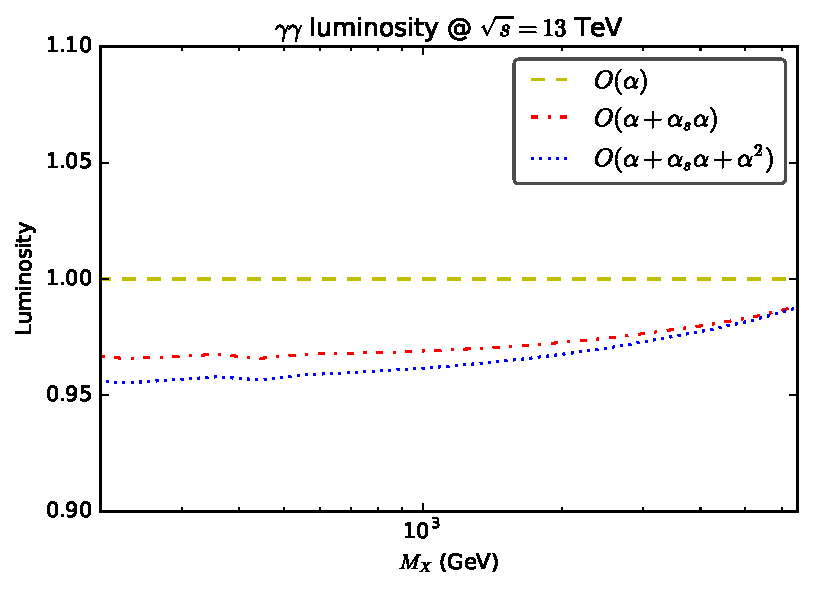
\includegraphics[width=8cm]{figs/lumi_13tev.pdf} 
\caption{The photon-photon
PDF luminosity $\mathcal{L}_{\gamma\gamma}$ at $\sqrt{s} = 13$ TeV as a
  function of the final state invariant mass $M_X$.
  %
  We compare the results of the photon evolved
  with only $\mathcal{O}(\alpha)$ corrections
  with the corresponding results with either
  $\mathcal{O}(\alpha+\alpha_s\alpha)$
  or $\mathcal{O}(\alpha+\alpha_s\alpha+\alpha^2)$ effects,
  normalized to the $\mathcal{O}(\alpha)$ result.
  %
  The calculation has been performed with
  NNPDF3.0QED as input.
}
\label{fig:GammaGammaLumi}
\end{figure}
%%%%%%%%%%%%%%%%%%%%%%%%%%%%%%%%%%%%%%%%%%%%%%%%%%%%%%%%

Fig.~\ref{fig:GammaGammaLumi} shows the behaviour of
$\Phi_{\gamma\gamma}$ computed using the photon PDF $\gamma$ of the
{\tt NNPDF30\_nlo\_as\_0118} PDF set evolved from $Q_0 = 1$ GeV to
$M_X$ including, on top of the pure QCD NLO evolution: only the LO QED
corrections $\mathcal{O}(\alpha)$ (yellow curve), also the mixed
corrections $\mathcal{O}(\alpha_s\alpha)$ (red curve), the full NLO
QCD+QED corrections, $i.e$
$\mathcal{O}(\alpha+\alpha_s\alpha+\alpha^2)$, (blue curve). All
predictions are normalized to the yellow curve. The
$\mathcal{O}(\alpha_s\alpha)$ and $\mathcal{O}(\alpha^2)$ corrections
have a small but non-negligible impact on the
$\gamma\gamma$-luminosity. In particular, these corrections suppress
$\Phi_{\gamma\gamma}$ by almost 5\% at relatively small values of
$M_X$, while the suppression gradually shrinks to 1-2\% as $M_X$
increases. As expected, most of the effect is ascribable to the
$\mathcal{O}(\alpha_s\alpha)$ corrections, while the
$\mathcal{O}(\alpha^2)$ ones have a substantially smaller impact.

\subsection{DIS structure functions}

When considering NLO QCD+QED corrections to the DIS structure
functions, one has to include into the hard cross sections all the
$\mathcal{O}(\alpha)$ diagrams where one photon is either in the
initial state or emitted from an incoming quark (or possibly an
incoming lepton). Such diagrams are of purely QED origin and no QCD
contributions are present. As a consequence, the corresponding
coefficient functions can easily be derived from the QCD expressions
just by properly adjusting the colour factors. In addition, this
correspondence holds regardless of whether mass effects are included
or not.

The main complication arises from the flavour structure. In fact, due
to the fact that the coupling of the photon is proportional to the
squared charge of the parton to which it couples (a quark or a
lepton), in the case of quarks the isospin symmetry is broken. In the
following we will address the case of Neutral-Current (NC), where
lepton and proton exchange a neutral boson $\gamma^*/Z$, and
Charged-Current (CC) structure functions separately, where instead
lepton and proton exchange a charged $W$ boson.

\subsubsection{NC structure functions}

In this section we concentrate on the $\mathcal{O}(\alpha)$
contributions to the generic NC structure function $F$. Due to the
fact that to this order there is no mixing between QCD and QED
couplings, such corrections can easily be derived from the structure
of the $\mathcal{O}(\alpha_s)$ corrections. The procedure is very
simple and it amounts of adjusting the colour factors by setting
$C_F=T_R=1$ and $C_A=0$ in the $\mathcal{O}(\alpha_s)$
expressions. Referring $e.g.$ to the expressions reported in
Ref.~\cite{Ellis:1991qj}, one simply has:
\begin{equation}\label{eq:alphaCFs}
\begin{array}{rcl}
\displaystyle C_{i;q}^{(\alpha)} &=& \displaystyle \frac{C_{i;q}^{(\alpha_s)}}{C_F}\\
\\
\displaystyle C_{i;\gamma}^{(\alpha)} &=& \displaystyle \frac{C_{i;g}^{(\alpha_s)}}{T_R}
\end{array}\quad i = 2,L,3\,.
\end{equation}
In addition, for constructing the corresponding structure functions,
considering that the coupling between a photon and a quark of flavour
$q$ is proportional to $e_q^2$, one also needs to adjust the couplings
by using:
 \begin{equation}
\begin{array}{rcl}
\widetilde{B}_q(Q) &=& B_q(Q)e_q^2\quad\mbox{for}\quad F_2,F_L\,, \\
\\
\widetilde{D}_q(Q) &=& D_q(Q)e_q^2\quad\mbox{for}\quad F_3\,, \\
\end{array}
\end{equation}
where $B_q(Q)$ and $D_q(Q)$ are the NC couplings (see $e.g.$
Ref.~\cite{Adloff:2003uh}). With these simple rules at hand, one can
write the $\mathcal{O}(\alpha)$ contributions to the NC structure
functions as:
\begin{equation}
\begin{array}{rcl}
F_{2,L}^{{\rm NC},(\alpha)} &=& \displaystyle x \sum_{q} \widetilde{B}_q\left[C_{2,L;q}^{(\alpha)}\otimes
(q+\overline{q}) + C_{2,L;\gamma}^{(\alpha)} \otimes \gamma
                         \right]\,,\\
\\
F_3^{{\rm NC},(\alpha)} &=& \displaystyle x \sum_{q} \widetilde{D}_q\left[C_{3;q}^{(\alpha)}\otimes
(q-\overline{q}) + C_{3;\gamma}^{(\alpha)} \otimes \gamma
                         \right]\,.
\end{array}
\end{equation}

It is important to notice that the same structure holds for both
massless and massive structure functions. This is relevant for the
construction of the FONLL structure functions.

\subsubsection{CC structure functions}

The CC case the procedure to obtain the expressions of the
$\mathcal{O}(\alpha)$ is exactly the same of the NC case, that is
eq.~(\ref{eq:alphaCFs}). However, this case is more complicated
because the flavour structure of the respective structure functions is
more complex. Taking into account the presence of a factor $e_q^2$
every time that a quark of flavour $q$ couples to the photon, the CC
structure functions $F_2$ and $F_L$ for the productions of a neutrino
or an anti-neutrino take the form:
\begin{equation}\label{compactNu}
\begin{array}{rcl}
F_{2,L}^{{\rm CC},\nu,(\alpha)} &=& \displaystyle
                              \sum_{U=u,c,t}\sum_{D=d,s,b}|V_{UD}|^2\left[C_{2,L;q}^{(\alpha)}\otimes\left(e_D^2D +e_U^2\overline{U}\right) +2 C_{2,L;\gamma}^{(\alpha)}\otimes\gamma\right]\,,\\
\\
F_{2,L}^{{\rm CC},\overline{\nu},(\alpha)} &=& \displaystyle
\sum_{U=u,c,t}\sum_{D=d,s,b}|V_{UD}|^2\left[C_{2,L;q}^{(\alpha)}\otimes\left(e_D^2\overline{D}
    +e_U^2U\right) +2 C_{2,L;\gamma}^{(\alpha)}\otimes\gamma\right]\,,
\end{array}
\end{equation}
where $V_{UD}$ are the elements of the CKM matrix. The flavour
structure for $F_3$ instead look slightly different:
\begin{equation}\label{compactNuF3}
\begin{array}{rcl}
F_3^{{\rm CC},\nu,(\alpha)} &=& \displaystyle
                              \sum_{U=u,c,t}\sum_{D=d,s,b}|V_{UD}|^2\left[C_{3;q}^{(\alpha)}\otimes\left(e_D^2D -e_U^2\overline{U}\right) +2 C_{3;\gamma}^{(\alpha)}\otimes\gamma\right]\,,\\
\\
F_3^{{\rm CC},\overline{\nu},(\alpha)} &=& \displaystyle
\sum_{U=u,c,t}\sum_{D=d,s,b}|V_{UD}|^2\left[C_{3;q}^{(\alpha)}\otimes\left(-e_D^2\overline{D}
    +e_U^2U\right) +2 C_{3;\gamma}^{(\alpha)}\otimes\gamma\right]\,,
\end{array}
\end{equation}

As mentioned above, the flavour structure of the CC structure
functions is more complex. This is the consequence of the introduction
of the QED isospin symmetry breaking associated to the mixing produced
by the CKM matrix. In order to simplify the implementation, it is of
great advantage to approximate the CKM matrix as a 3 by 3 unitary
matrix. The inaccuracy introduced in doing so is of the order of
$\alpha$ times the value of off-diagonal elements of the CKM matrix
and thus it is expected to be very small.

As an illustration of the impact of the $\mathcal{O}(\alpha)$
correction on the DIS structure functions, Fig.~\ref{fig:StructFuncs}
shows the effect of introducing these contributions on the pure QCD
computation at NLO. The plots are produced by evolving the {\tt
  NNPDF30\_nlo\_as\_0118\_qed} PDF set~\cite{Bertone:2016ume} from 1
GeV to 100 GeV including the NLO CD+QED corrections discussed in the
previous section and using the resulting evolved PDFs to compute the
NC (left panel) and the CC (right panel) DIS structure functions in
the FONLL-B scheme (NLO) including the $\mathcal{O}(\alpha)$
corrections to the coefficient functions discussed above. The
predictions are shown normalised to the pure QCD computation where the
QED corrections are absent both in the evolution and in the
computation of the structure functions.

%%%%%%%%%%%%%%%%%%%%%%%%%%%%%%%%%%%%%%%%%%%%%%%%%%%%%%%%
\begin{figure}[t]
\includegraphics[width=6cm,angle=270]{figs/NLOQEDCorrections_NC.eps}
\includegraphics[width=6cm,angle=270]{figs/NLOQEDCorrections_CC.eps}
\caption{The effects of NLO QED corrections on the neutral-current
(left) and charged-current (right) DIS structure functions
$F_2, F_3$ and $F_L$, normalized to the pure QCD result.
%
The calculation has been performed with the NNPDF3.0QED NLO
set in the FONLL-B general-mass scheme.
%
Note that QED effects enter both via modified DGLAP
evolution and the photon-induced DIS coefficient
functions.
}
\label{fig:StructFuncs}
\end{figure}
%%%%%%%%%%%%%%%%%%%%%%%%%%%%%%%%%%%%%%%%%%%%%%%%%%%%%%%%

It is clear that the impact of the full NLO QCD+QED corrections is
pretty small especially in the low-$x$ region where QCD dominates and
the impact of the QED contributions is well below 1\%. In the
large-$x$ region, instead, the presence of a contribution proportional
to the photon PDF is more significant because of the relative
suppression of the QCD distributions (quarks and gluon) and the impact
of the QED corrections reaches the 2\% level.  It should be stressed
that the behaviour around $x=10^{-2}$ of the CC $F_3$ (green curve in
the right panel) is driven by a change of sign of the predictions so
that the ratio diverges.

